\documentclass[aspectratio=43]{beamer}
	\usepackage{tikz}
	\usepackage{tikz-cd}

	\usetikzlibrary{calc}
	\usetikzlibrary{fadings}
	\usetikzlibrary{shapes.geometric, arrows, positioning}

	\tikzstyle{layerheader} = [rectangle, minimum width=3cm, minimum height=1cm, text centered, draw=black, fill=gray!30]
	\tikzstyle{startstop} = [ellipse, minimum width=3cm, minimum height=1cm, text centered, draw=black, fill=red!30]
	\tikzstyle{process} = [rectangle, minimum width=3cm, minimum height=1cm, text centered, draw=black, fill=blue!20]
	\tikzstyle{decision} = [diamond, minimum width=2.5cm, minimum height=1cm, text centered, draw=black, fill=green!20]
	\tikzstyle{arrow} = [thick,->,>=stealth]

\usetheme{Berlin}
\usepackage[czech]{babel}
\usecolortheme{dolphin}
\usepackage{graphicx}
\usepackage{dirtree}
\usepackage{listings}
\usepackage[T1]{fontenc}
\usepackage{lmodern}
\usepackage[utf8]{inputenc}
\usepackage{caption}
\usepackage{bbding}
\usepackage{xurl}
\usepackage{scrextend}
\usepackage{appendixnumberbeamer}


\captionsetup{labelformat=empty}

\beamertemplatenavigationsymbolsempty
\defbeamertemplate*{title page}{customized}[1][]
{
	\usebeamerfont{title}\inserttitle\par
	% \usebeamerfont{subtitle}\usebeamercolor[fg]{subtitle}\insertsubtitle\par
	\bigskip
	\usebeamerfont{author}\insertauthor\par
	\usebeamerfont{institute}\insertinstitute\par
	\usebeamerfont{date}\insertdate\par
	\usebeamercolor[fg]{titlegraphic}\inserttitlegraphic
}

\hypersetup{unicode}
\hypersetup{breaklinks=true}


\title{FMCW surveillance radar}
% \subtitle{----}
\author{Havránek Kryštof}
\date{June 2025}
\institute{České vysoké učení technické v Praze}
\setbeamertemplate{sidebar right}{}
\setbeamertemplate{footline}{%
\hfill\textbf{\insertframenumber{}/\inserttotalframenumber} \hspace{0.01cm} \vspace{0.1cm}}
\setbeamerfont{footnote}{size=\tiny}

\begin{document}

\begin{frame}[plain]
  \maketitle
\end{frame}

\clearpage
\setcounter{framenumber}{0}

\begin{frame}[fragile]
  \frametitle{Sections}

  \begin{enumerate}
    \item Surveillance FMCW radar
    \item SiRad Easy
    \item Rotary Platform
    \item Desktop Application
    \item Conclusion
  \end{enumerate}
\end{frame}


\begin{frame}[fragile]
  \frametitle{Surveillance Radar}
  \section{FMCW Radar}

  \begin{itemize}
    \item Detection of target in 2D/3D space
    \item 2 basic approaches
      \begin{itemize}
        \item MIMO systems - electronic beamsteering, complex processing, preferred for demanding applications
        \item Mechanical scanning - simpler, easier processing, cheaper, mechanical components
      \end{itemize}
    \item Generally based on pulsed radars
			\begin{itemize}
				\item Distance from RTT, speed from Doppler
				\item Require high broadcast power for high resolution
			\end{itemize}
  \end{itemize}
\end{frame}


\begin{frame}[fragile]
  \frametitle{FMCW Radar}

  \begin{figure}[h!]
    \centering
    \begin{tikzpicture}[>=latex, scale=0.6]

      % Axes
      \draw[->] (0, 0) -- (8, 0) node[below] {$t$};
      \draw[->] (0, 0) -- (0, 5) node[left] {$f$};

      % Horizontal lines for BW
      \draw[dashed] (0, 4.5) -- (7.5, 4.5);
      \draw[dashed] (0, 1) -- (7.5, 1);
      \draw[dashed] (2.5, -0.05) -- (2.5, 4.7);

      % Labels for fc and BW
      \node[left] at (0, 0.7) {$f_c$};
      \draw[<->] (-0.5, 1) -- (-0.5, 4.5) node[midway,left] {$BW$};

      % Triangular wave for Tx
      \draw[thick,blue] (0, 1) -- (2.5, 4.5);
      \draw[thick,blue]	(2.5, 1) -- (5, 4.5);
      \draw[thick, dashed, blue] (5, 1) -- (6, 2.4);

      % Triangular wave for Rx (offset version)
      \draw[thick,red] (0.5, 1) -- (3, 4.5);
      \draw[thick,red] (3, 1) -- (5.5, 4.5);
      \draw[thick, dashed, red] (5.4, 1) -- (6.4, 2.4);

      % Label for Tch
      \draw[-] (2.5, -0.05) -- (2.5, 0.05) node[below] {$T_{\text{ch}}$};

      % Labels for Tx and Rx
      \node[blue] at (4.2, 4.1) {\small Tx};
      \node[red] at (5.3, 3.7) {\small Rx};

      % Sweep slope and fb
      \draw[<->] (1, 1) arc[start angle=0, end angle=55, radius=1];
      \node at (1.5, 1.3) {\small $k_{\text{sw}}$};
      \draw[<->] (1.5, 2.37) -- (1.5, 3.12) node[above, left] {$f_b$};

      % Small time delay (tau)
      \draw[<->] (2.5, 0.7) -- (3, 0.7) node[midway,below] {$\tau$};

    \end{tikzpicture}

    \caption{Ideal relation of frequency on time for received and sent signal}
    \label{fig:fmcw_ideal}
  \end{figure}
  \begin{itemize}
    \item Broadcasts frequency modulated signal
    \item Low power consumption with great ranger resolution
    \item Range of target: $R = \frac{c_0 f_\mathrm{b} T_\mathrm{ch}}{2BW}$, $\Delta R = \frac{c_0 N_\mathrm{samples}}{2BW \cdot NFFT}$
    \item Speed of target: causes phase shift across many chirps
  \end{itemize}
\end{frame}

\begin{frame}[fragile]
  \frametitle{SiRad Easy}
  \section{SiRad Easy}

  \begin{figure}[h!]
    \centering
    \includegraphics[width=0.5\textwidth]{../img/sirad.png}

    \caption{SiRad Easy  24~GHz configuration }
    \label{fig:sirad}
  \end{figure}

  \begin{itemize}
    \item Evaluation kit from Indie Semiconductors
    \item Supports 24~GHz and 122~GHz transceivers
    \item Primarily designed to supply already processed data
  \end{itemize}
\end{frame}

\begin{frame}[fragile]
  \frametitle{SiRad Easy}

  \begin{itemize}
    \item Slow update rate (at best around 20~ms)
      \begin{itemize}
        \item Maximal detectable speed bellow 1~ms/s
        \item Rotation speed limited to low RPM
      \end{itemize}
    \item 122~GHz header
      \begin{itemize}
        \item Tight radar beam $\pm 4$° in both directions
        \item Maximal advertised ranged of 40~m, measured one closed to 30~m
        \item Ideal for close range, high resolution applications
      \end{itemize}
  \end{itemize}
\end{frame}

\begin{frame}[fragile]
  \frametitle{SiRad Easy}

  \begin{figure}[h!]
    \centering
    \includegraphics[width=0.43\textwidth]{../img/farfield3d.png}
    \caption{Radiation pattern of 24~GHz header -- 3D view}
    \label{fig:farfield3d}
  \end{figure}

  \begin{itemize}
    \item 24~GHz header
      \begin{itemize}
        \item Radiation characteristics simulated in CST studio
        \item 16 degrees in azimuth, 30 degrees in elevation
        \item Long range applications
      \end{itemize}
  \end{itemize}
\end{frame}


\begin{frame}[fragile]
  \frametitle{Rotary Platform}
  \section{Rotary Platform}
  \begin{figure}[!htb]
    \begin{minipage}{0.48\textwidth}
      \begin{itemize}
        \item Two axis of movement
        \item Continuos rotation with aid of a slipring
        \item Powered by ESP32C6 microcontroller
        \item G-Code-like API
        \item Supports: automatic homing, relative/absolute positioning, spindle, preprogramming movement sequence
      \end{itemize}
    \end{minipage}\hfill
    \begin{minipage}{0.48\textwidth}
      \centering
      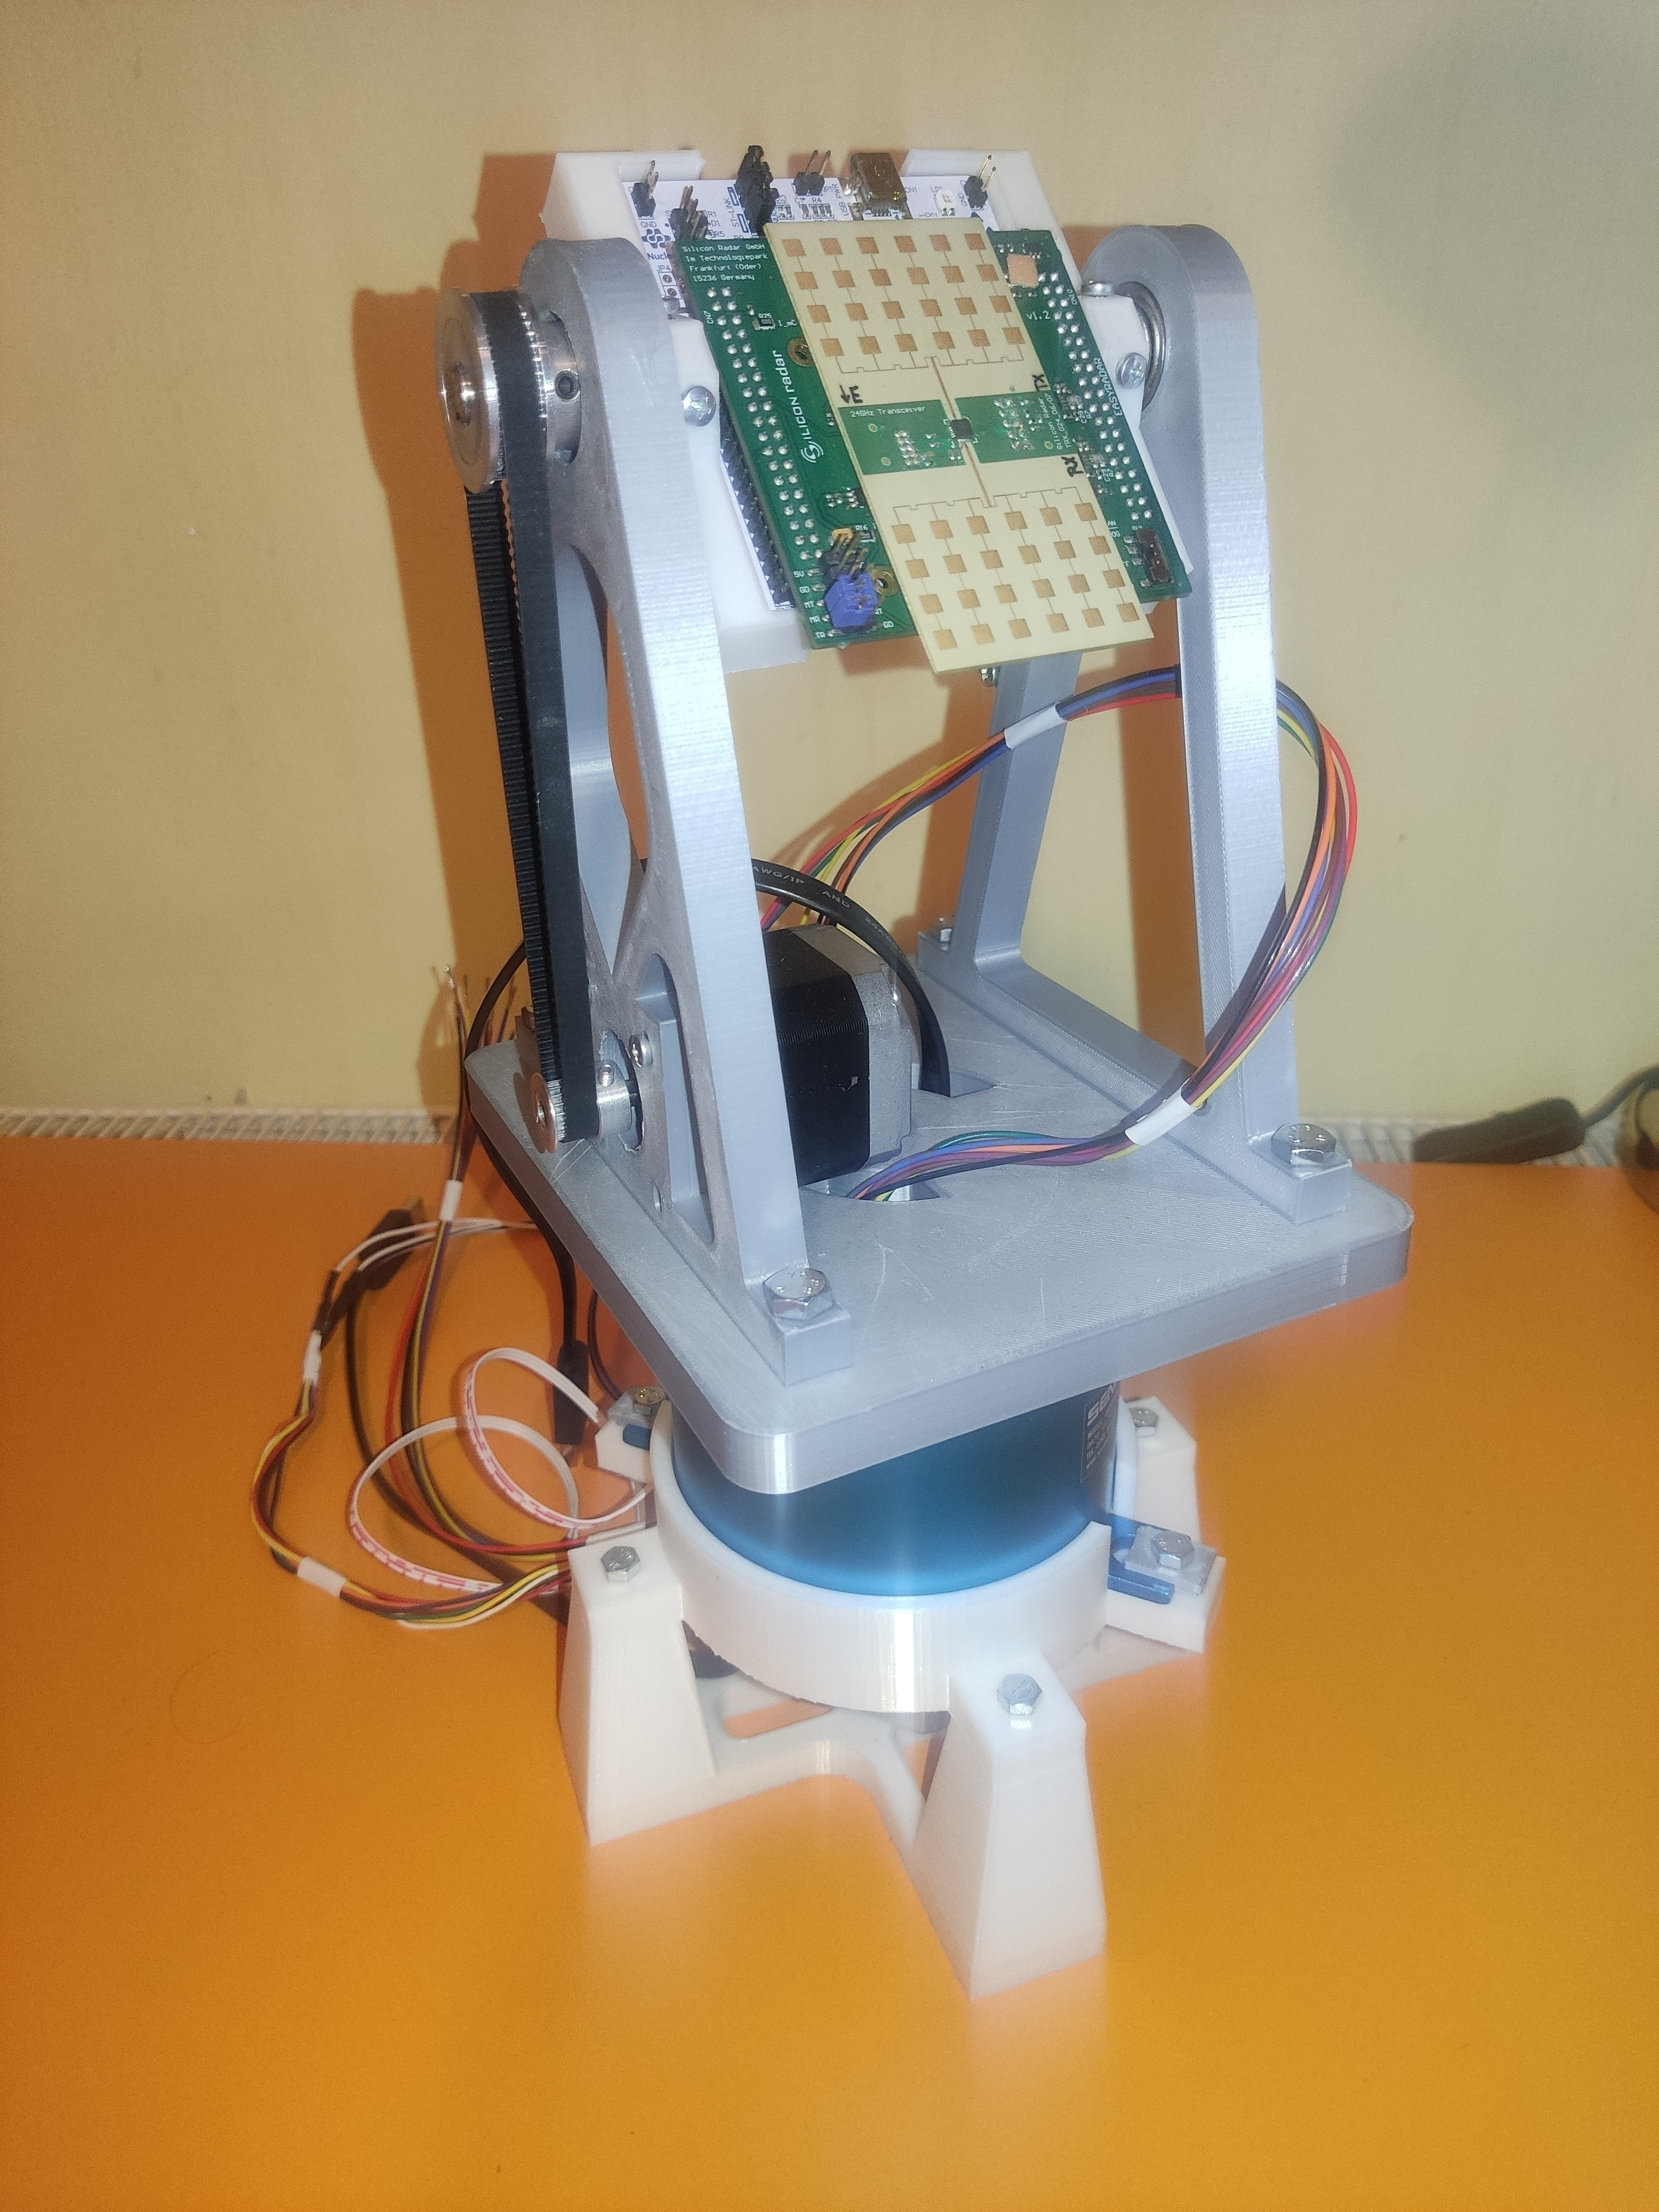
\includegraphics[width=.8\linewidth]{../img/assembly_photo.jpg}
      \caption{Platform}
    \end{minipage}
  \end{figure}
\end{frame}

\begin{frame}[fragile]
  \frametitle{Platform Firmware Flow}

  \centering
  \includegraphics[width=0.75\textwidth]{../img/platform_flow.jpg}

\end{frame}

\begin{frame}[fragile]
  \frametitle{Platform Program Example}
  \begin{tabular}{lll}
    \hline
    \texttt{Command}     & Mode   & Purpose                      \\
    \hline
    \texttt{P90 rotTilt} & Header & Initialize program rotTilt   \\
    \texttt{G91}         & Header & Set relative positioning     \\
    \texttt{G21}         & Header & Set units to steps           \\
    \texttt{G28}         & Header & Start auto home routine      \\
    \texttt{G0 P-50 S6}  & Header & Move pitch 50 steps          \\
    \texttt{W3 T5000}    & Header & Wait five second             \\
    \texttt{P92}         & Header & Set current position as home \\
    \texttt{P29}         & Header & Enable infinite looping      \\
    \texttt{M03 SY6 Y+}  & Header & Start Yaw spindle (6 RPM)    \\
    \texttt{P92}         & Header & Finalize header declaration  \\
    \texttt{G0 S5 P40}   & Body   & Pitch movement               \\
    \texttt{G0 S5 P-40}  & Body   & Return pitch                 \\
    \texttt{P92}         & Body   & Finalize program             \\
    \hline
  \end{tabular}
\end{frame}




\begin{frame}[fragile]
  \frametitle{Desktop Application}
  \section{Desktop Application}

  \begin{figure}[h!]
    \centering
    \includegraphics[width=0.7\textwidth]{../img/vis_range_azimuth.jpg}
    \caption[]{Range-Azimuth visualization}
  \end{figure}

  \begin{itemize}
    \item Control app written in MATLAB
    \item Integrates radar and platform data
    \item Offers wide degree of customization
  \end{itemize}
\end{frame}

\begin{frame}[fragile]
  \frametitle{Preferences: Radar}
  \begin{center}
    \includegraphics[width=0.9\textwidth]{../img/preferences_crop1.jpg}
  \end{center}
\end{frame}

\begin{frame}[fragile]
  \frametitle{Preferences: Processing}
  \begin{center}
    \includegraphics[width=0.9\textwidth]{../img/preferences_crop2.jpg}
  \end{center}
\end{frame}

\begin{frame}[fragile]
  \frametitle{Data Aquisition}
  \begin{center}
    \includegraphics[width=0.8\textwidth]{../img/dataflow_1.jpg}
  \end{center}
\end{frame}

\begin{frame}[fragile]
  \frametitle{Data Processing}
  \begin{center}
    \includegraphics[width=0.8\textwidth]{../img/dataflow_2.jpg}
  \end{center}
\end{frame}

\begin{frame}[fragile]
  \frametitle{Data Storing}
  \begin{center}
    \includegraphics[width=0.7\textwidth]{../img/dataflow_3.jpg}
  \end{center}
\end{frame}

\begin{frame}[fragile]
  \frametitle{Visualization}
  \begin{itemize}
    \item Data are only provided in graphic way to the user
    \item Simple storage method allows for easy integration of other visualization methods
    \item Three visualization styles
      \begin{itemize}
        \item Range-RCS or Range-Doppler
        \item Range-Azimuth
        \item 3D
      \end{itemize}
  \end{itemize}
\end{frame}


\begin{frame}[fragile]
  \frametitle{Visualization: Range-RCS/Doppler}
  \begin{figure}[!htb]
    \begin{minipage}{0.48\textwidth}
      \centering
      \includegraphics[width=\textwidth]{../img/vis_range_dop.jpg}
      \caption{Range-Doppler}
    \end{minipage}\hfill
    \begin{minipage}{0.48\textwidth}
      \centering
      \includegraphics[width=\textwidth]{../img/vis_range_rcs.jpg}
      \caption{Ranger-RCS}
    \end{minipage}
  \end{figure}
\end{frame}

\begin{frame}[fragile]
  \frametitle{Visualizatio: 3D}
  \begin{center}
    \includegraphics[width=0.9\textwidth]{../img/vis_3d.jpg}
  \end{center}
\end{frame}


\begin{frame}[fragile]
  \frametitle{Conclusion}
  \section{Conclusion}
  \begin{itemize}
    \item SiRad Easy
      \begin{itemize}
        \item Sufficient for monitoring static scenes
        \item Speed estimation is limited -- tracking application isn't a possibility
      \end{itemize}
    \item Rotary platform
      \begin{itemize}
        \item Matches design requirements
        \item Underpowered azimuth motor and low belt tension
      \end{itemize}
		\item Desktop application
			\begin{itemize}
				\item Large degree of configuration
				\item Pipeline performant, except final visualization under Linux
			\end{itemize}
  \end{itemize}
\end{frame}



\begin{frame}[fragile]
  \frametitle{Q1: Exprimental Data}

  \begin{itemize}
    \item Large number of parameters: header, bandwidth, gain, target, CFAR setting -- requires fine tuning
		\item Rotary movement + inconsistent radar timing complicate reproducibility
    \item Author couldn't establish correct, reproducible, validation methodology to give measured data any validity
    \item No testing in controlled environment was done
    \item When static the radar capabilities generally match advertised
      \begin{itemize}
        \item 122~GHz header -- Tight beam $\Rightarrow$ very sensitive to target orientation
      \end{itemize}
  \end{itemize}
\end{frame}



\end{document}


% Software běžící na mikrokontroléru je relativně přímočarý.
%


% Kvůli relativně obecnému zadání má aplikaci celou řadu nastavitelných paramterů
%
% Zpracování dat začíná vyčtením dat z radaru
%
%
% Po tomto krotku má program dva objekty - pole cílů z CFAR a range-Doppler mapu
%
%
% je li vyrovávací pamět plná, spustí se update radarové kostky v paralelním vlákně.
% Radar cube je základní datová struktura, která uchovává informace o prostoru v n dimenzionálnách polích.
%
% Takové kostky jsou v paměti dvě - jedna pro surová data, druhá pro CFAR výstup.
% Proces je paralelizován jelikož systém podporuje postupné stárnutí dat, což vyžaduje stovky tisíc floating point operací u větších kostek
%
%
% Shrnuto.
%
%
